\documentclass[1p]{elsarticle_modified}
%\bibliographystyle{elsarticle-num}

%\usepackage[colorlinks]{hyperref}
%\usepackage{abbrmath_seonhwa} %\Abb, \Ascr, \Acal ,\Abf, \Afrak
\usepackage{amsfonts}
\usepackage{amssymb}
\usepackage{amsmath}
\usepackage{amsthm}
\usepackage{scalefnt}
\usepackage{amsbsy}
\usepackage{kotex}
\usepackage{caption}
\usepackage{subfig}
\usepackage{color}
\usepackage{graphicx}
\usepackage{xcolor} %% white, black, red, green, blue, cyan, magenta, yellow
\usepackage{float}
\usepackage{setspace}
\usepackage{hyperref}

\usepackage{tikz}
\usetikzlibrary{arrows}

\usepackage{multirow}
\usepackage{array} % fixed length table
\usepackage{hhline}

%%%%%%%%%%%%%%%%%%%%%
\makeatletter
\renewcommand*\env@matrix[1][\arraystretch]{%
	\edef\arraystretch{#1}%
	\hskip -\arraycolsep
	\let\@ifnextchar\new@ifnextchar
	\array{*\c@MaxMatrixCols c}}
\makeatother %https://tex.stackexchange.com/questions/14071/how-can-i-increase-the-line-spacing-in-a-matrix
%%%%%%%%%%%%%%%

\usepackage[normalem]{ulem}

\newcommand{\msout}[1]{\ifmmode\text{\sout{\ensuremath{#1}}}\else\sout{#1}\fi}
%SOURCE: \msout is \stkout macro in https://tex.stackexchange.com/questions/20609/strikeout-in-math-mode

\newcommand{\cancel}[1]{
	\ifmmode
	{\color{red}\msout{#1}}
	\else
	{\color{red}\sout{#1}}
	\fi
}

\newcommand{\add}[1]{
	{\color{blue}\uwave{#1}}
}

\newcommand{\replace}[2]{
	\ifmmode
	{\color{red}\msout{#1}}{\color{blue}\uwave{#2}}
	\else
	{\color{red}\sout{#1}}{\color{blue}\uwave{#2}}
	\fi
}

\newcommand{\Sol}{\mathcal{S}} %segment
\newcommand{\D}{D} %diagram
\newcommand{\A}{\mathcal{A}} %arc


%%%%%%%%%%%%%%%%%%%%%%%%%%%%%5 test

\def\sl{\operatorname{\textup{SL}}(2,\Cbb)}
\def\psl{\operatorname{\textup{PSL}}(2,\Cbb)}
\def\quan{\mkern 1mu \triangleright \mkern 1mu}

\theoremstyle{definition}
\newtheorem{thm}{Theorem}[section]
\newtheorem{prop}[thm]{Proposition}
\newtheorem{lem}[thm]{Lemma}
\newtheorem{ques}[thm]{Question}
\newtheorem{cor}[thm]{Corollary}
\newtheorem{defn}[thm]{Definition}
\newtheorem{exam}[thm]{Example}
\newtheorem{rmk}[thm]{Remark}
\newtheorem{alg}[thm]{Algorithm}

\newcommand{\I}{\sqrt{-1}}
\begin{document}

%\begin{frontmatter}
%
%\title{Boundary parabolic representations of knots up to 8 crossings}
%
%%% Group authors per affiliation:
%\author{Yunhi Cho} 
%\address{Department of Mathematics, University of Seoul, Seoul, Korea}
%\ead{yhcho@uos.ac.kr}
%
%
%\author{Seonhwa Kim} %\fnref{s_kim}}
%\address{Center for Geometry and Physics, Institute for Basic Science, Pohang, 37673, Korea}
%\ead{ryeona17@ibs.re.kr}
%
%\author{Hyuk Kim}
%\address{Department of Mathematical Sciences, Seoul National University, Seoul 08826, Korea}
%\ead{hyukkim@snu.ac.kr}
%
%\author{Seokbeom Yoon}
%\address{Department of Mathematical Sciences, Seoul National University, Seoul, 08826,  Korea}
%\ead{sbyoon15@snu.ac.kr}
%
%\begin{abstract}
%We find all boundary parabolic representation of knots up to 8 crossings.
%
%\end{abstract}
%\begin{keyword}
%    \MSC[2010] 57M25 
%\end{keyword}
%
%\end{frontmatter}

%\linenumbers
%\tableofcontents
%
\newcommand\colored[1]{\textcolor{white}{\rule[-0.35ex]{0.8em}{1.4ex}}\kern-0.8em\color{red} #1}%
%\newcommand\colored[1]{\textcolor{white}{ #1}\kern-2.17ex	\textcolor{white}{ #1}\kern-1.81ex	\textcolor{white}{ #1}\kern-2.15ex\color{red}#1	}

{\Large $\underline{12a_{0203}~(K12a_{0203})}$}

\setlength{\tabcolsep}{10pt}
\renewcommand{\arraystretch}{1.6}
\vspace{1cm}\begin{tabular}{m{100pt}>{\centering\arraybackslash}m{274pt}}
\multirow{5}{120pt}{
	\centering
	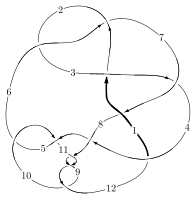
\includegraphics[width=112pt]{../../../GIT/diagram.site/Diagrams/png/1004_12a_0203.png}\\
\ \ \ A knot diagram\footnotemark}&
\allowdisplaybreaks
\textbf{Linearized knot diagam} \\
\cline{2-2}
 &
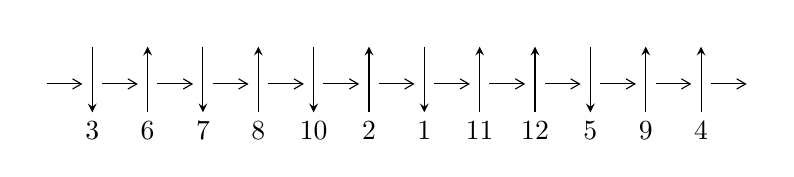
\begin{tikzpicture}[x=20pt, y=17pt]
	% nodes
	\node (C0) at (0, 0) {};
	\node (C1) at (1, 0) {};
	\node (C1U) at (1, +1) {};
	\node (C1D) at (1, -1) {3};

	\node (C2) at (2, 0) {};
	\node (C2U) at (2, +1) {};
	\node (C2D) at (2, -1) {6};

	\node (C3) at (3, 0) {};
	\node (C3U) at (3, +1) {};
	\node (C3D) at (3, -1) {7};

	\node (C4) at (4, 0) {};
	\node (C4U) at (4, +1) {};
	\node (C4D) at (4, -1) {8};

	\node (C5) at (5, 0) {};
	\node (C5U) at (5, +1) {};
	\node (C5D) at (5, -1) {10};

	\node (C6) at (6, 0) {};
	\node (C6U) at (6, +1) {};
	\node (C6D) at (6, -1) {2};

	\node (C7) at (7, 0) {};
	\node (C7U) at (7, +1) {};
	\node (C7D) at (7, -1) {1};

	\node (C8) at (8, 0) {};
	\node (C8U) at (8, +1) {};
	\node (C8D) at (8, -1) {11};

	\node (C9) at (9, 0) {};
	\node (C9U) at (9, +1) {};
	\node (C9D) at (9, -1) {12};

	\node (C10) at (10, 0) {};
	\node (C10U) at (10, +1) {};
	\node (C10D) at (10, -1) {5};

	\node (C11) at (11, 0) {};
	\node (C11U) at (11, +1) {};
	\node (C11D) at (11, -1) {9};

	\node (C12) at (12, 0) {};
	\node (C12U) at (12, +1) {};
	\node (C12D) at (12, -1) {4};
	\node (C13) at (13, 0) {};

	% arrows
	\draw[->,>={angle 60}]
	(C0) edge (C1) (C1) edge (C2) (C2) edge (C3) (C3) edge (C4) (C4) edge (C5) (C5) edge (C6) (C6) edge (C7) (C7) edge (C8) (C8) edge (C9) (C9) edge (C10) (C10) edge (C11) (C11) edge (C12) (C12) edge (C13) ;	\draw[->,>=stealth]
	(C1U) edge (C1D) (C2D) edge (C2U) (C3U) edge (C3D) (C4D) edge (C4U) (C5U) edge (C5D) (C6D) edge (C6U) (C7U) edge (C7D) (C8D) edge (C8U) (C9D) edge (C9U) (C10U) edge (C10D) (C11D) edge (C11U) (C12D) edge (C12U) ;
	\end{tikzpicture} \\
\hhline{~~} \\& 
\textbf{Solving Sequence} \\ \cline{2-2} 
 &
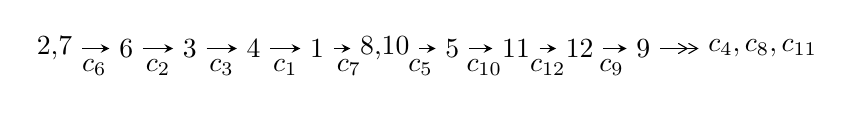
\begin{tikzpicture}[x=23pt, y=7pt]
	% node
	\node (A0) at (-1/8, 0) {2,7};
	\node (A1) at (1, 0) {6};
	\node (A2) at (2, 0) {3};
	\node (A3) at (3, 0) {4};
	\node (A4) at (4, 0) {1};
	\node (A5) at (81/16, 0) {8,10};
	\node (A6) at (49/8, 0) {5};
	\node (A7) at (57/8, 0) {11};
	\node (A8) at (65/8, 0) {12};
	\node (A9) at (73/8, 0) {9};
	\node (C1) at (1/2, -1) {$c_{6}$};
	\node (C2) at (3/2, -1) {$c_{2}$};
	\node (C3) at (5/2, -1) {$c_{3}$};
	\node (C4) at (7/2, -1) {$c_{1}$};
	\node (C5) at (9/2, -1) {$c_{7}$};
	\node (C6) at (45/8, -1) {$c_{5}$};
	\node (C7) at (53/8, -1) {$c_{10}$};
	\node (C8) at (61/8, -1) {$c_{12}$};
	\node (C9) at (69/8, -1) {$c_{9}$};
	\node (A10) at (11, 0) {$c_{4},c_{8},c_{11}$};

	% edge
	\draw[->,>=stealth]	
	(A0) edge (A1) (A1) edge (A2) (A2) edge (A3) (A3) edge (A4) (A4) edge (A5) (A5) edge (A6) (A6) edge (A7) (A7) edge (A8) (A8) edge (A9) ;
	\draw[->>,>={angle 60}]	
	(A9) edge (A10);
\end{tikzpicture} \\ 

\end{tabular} \\

\footnotetext{
The image of knot diagram is generated by the software ``\textbf{Draw programme}" developed by Andrew Bartholomew(\url{http://www.layer8.co.uk/maths/draw/index.htm\#Running-draw}), where we modified some parts for our purpose(\url{https://github.com/CATsTAILs/LinksPainter}).
}\phantom \\ \newline 
\centering \textbf{Ideals for irreducible components\footnotemark of $X_{\text{par}}$} 
 
\begin{align*}
I^u_{1}&=\langle 
u^{99}+u^{98}+\cdots+b- u,\;- u^{99}+u^{98}+\cdots-2 u^2+a,\;u^{101}-2 u^{100}+\cdots-3 u+1\rangle \\
I^u_{2}&=\langle 
b+u,\;- u^3+a- u+1,\;u^4+u^2- u+1\rangle \\
I^u_{3}&=\langle 
- u^5- u^4-2 u^3-2 u^2+b-2 u-1,\;u^4+u^2+a,\;u^6+u^5+2 u^4+2 u^3+2 u^2+2 u+1\rangle \\
\\
\end{align*}
\raggedright * 3 irreducible components of $\dim_{\mathbb{C}}=0$, with total 111 representations.\\
\footnotetext{All coefficients of polynomials are rational numbers. But the coefficients are sometimes approximated in decimal forms when there is not enough margin.}
\newpage
\renewcommand{\arraystretch}{1}
\centering \section*{I. $I^u_{1}= \langle u^{99}+u^{98}+\cdots+b- u,\;- u^{99}+u^{98}+\cdots-2 u^2+a,\;u^{101}-2 u^{100}+\cdots-3 u+1 \rangle$}
\flushleft \textbf{(i) Arc colorings}\\
\begin{tabular}{m{7pt} m{180pt} m{7pt} m{180pt} }
\flushright $a_{2}=$&$\begin{pmatrix}0\\u\end{pmatrix}$ \\
\flushright $a_{7}=$&$\begin{pmatrix}1\\0\end{pmatrix}$ \\
\flushright $a_{6}=$&$\begin{pmatrix}1\\u^2\end{pmatrix}$ \\
\flushright $a_{3}=$&$\begin{pmatrix}u\\u^3+u\end{pmatrix}$ \\
\flushright $a_{4}=$&$\begin{pmatrix}- u^3\\u^3+u\end{pmatrix}$ \\
\flushright $a_{1}=$&$\begin{pmatrix}u^3\\u^5+u^3+u\end{pmatrix}$ \\
\flushright $a_{8}=$&$\begin{pmatrix}u^8+u^6+u^4+1\\u^{10}+2 u^8+3 u^6+2 u^4+u^2\end{pmatrix}$ \\
\flushright $a_{10}=$&$\begin{pmatrix}u^{99}- u^{98}+\cdots-4 u^3+2 u^2\\- u^{99}- u^{98}+\cdots-3 u^2+u\end{pmatrix}$ \\
\flushright $a_{5}=$&$\begin{pmatrix}u^{21}+4 u^{19}+9 u^{17}+12 u^{15}+12 u^{13}+10 u^{11}+9 u^9+6 u^7+3 u^5+u\\u^{23}+5 u^{21}+\cdots+2 u^3+u\end{pmatrix}$ \\
\flushright $a_{11}=$&$\begin{pmatrix}- u^{99}+u^{98}+\cdots+2 u-1\\u^{99}- u^{98}+\cdots+2 u^3-2 u^2\end{pmatrix}$ \\
\flushright $a_{12}=$&$\begin{pmatrix}- u^{11}-2 u^9-2 u^7+u^3\\u^{11}+3 u^9+4 u^7+3 u^5+u^3+u\end{pmatrix}$ \\
\flushright $a_{9}=$&$\begin{pmatrix}- u^{96}+u^{95}+\cdots-2 u^3+u\\- u^{98}+u^{97}+\cdots-2 u^2+u\end{pmatrix}$\\&\end{tabular}
\flushleft \textbf{(ii) Obstruction class $= -1$}\\~\\
\flushleft \textbf{(iii) Cusp Shapes $= -4 u^{100}+12 u^{99}+\cdots-27 u+14$}\\~\\
\newpage\renewcommand{\arraystretch}{1}
\flushleft \textbf{(iv) u-Polynomials at the component}\newline \\
\begin{tabular}{m{50pt}|m{274pt}}
Crossings & \hspace{64pt}u-Polynomials at each crossing \\
\hline $$\begin{aligned}c_{1}\end{aligned}$$&$\begin{aligned}
&u^{101}+48 u^{100}+\cdots+u-1
\end{aligned}$\\
\hline $$\begin{aligned}c_{2},c_{6}\end{aligned}$$&$\begin{aligned}
&u^{101}-2 u^{100}+\cdots-3 u+1
\end{aligned}$\\
\hline $$\begin{aligned}c_{3}\end{aligned}$$&$\begin{aligned}
&u^{101}+2 u^{100}+\cdots+12760 u+1480
\end{aligned}$\\
\hline $$\begin{aligned}c_{4}\end{aligned}$$&$\begin{aligned}
&u^{101}-2 u^{100}+\cdots-86401 u+194329
\end{aligned}$\\
\hline $$\begin{aligned}c_{5},c_{10}\end{aligned}$$&$\begin{aligned}
&u^{101}- u^{100}+\cdots-1024 u-1024
\end{aligned}$\\
\hline $$\begin{aligned}c_{7}\end{aligned}$$&$\begin{aligned}
&u^{101}-10 u^{100}+\cdots-42087 u+6643
\end{aligned}$\\
\hline $$\begin{aligned}c_{8},c_{9},c_{11}\end{aligned}$$&$\begin{aligned}
&u^{101}+11 u^{100}+\cdots-8 u-1
\end{aligned}$\\
\hline $$\begin{aligned}c_{12}\end{aligned}$$&$\begin{aligned}
&u^{101}+12 u^{100}+\cdots+3723 u+277
\end{aligned}$\\
\hline
\end{tabular}\\~\\
\newpage\renewcommand{\arraystretch}{1}
\flushleft \textbf{(v) Riley Polynomials at the component}\newline \\
\begin{tabular}{m{50pt}|m{274pt}}
Crossings & \hspace{64pt}Riley Polynomials at each crossing \\
\hline $$\begin{aligned}c_{1}\end{aligned}$$&$\begin{aligned}
&y^{101}+12 y^{100}+\cdots-7 y-1
\end{aligned}$\\
\hline $$\begin{aligned}c_{2},c_{6}\end{aligned}$$&$\begin{aligned}
&y^{101}+48 y^{100}+\cdots+y-1
\end{aligned}$\\
\hline $$\begin{aligned}c_{3}\end{aligned}$$&$\begin{aligned}
&y^{101}-24 y^{100}+\cdots+111920400 y-2190400
\end{aligned}$\\
\hline $$\begin{aligned}c_{4}\end{aligned}$$&$\begin{aligned}
&y^{101}-48 y^{100}+\cdots-26966856735 y-37763760241
\end{aligned}$\\
\hline $$\begin{aligned}c_{5},c_{10}\end{aligned}$$&$\begin{aligned}
&y^{101}+63 y^{100}+\cdots-4718592 y-1048576
\end{aligned}$\\
\hline $$\begin{aligned}c_{7}\end{aligned}$$&$\begin{aligned}
&y^{101}+24 y^{100}+\cdots-2017745343 y-44129449
\end{aligned}$\\
\hline $$\begin{aligned}c_{8},c_{9},c_{11}\end{aligned}$$&$\begin{aligned}
&y^{101}-99 y^{100}+\cdots-132 y^2-1
\end{aligned}$\\
\hline $$\begin{aligned}c_{12}\end{aligned}$$&$\begin{aligned}
&y^{101}+12 y^{100}+\cdots+194657 y-76729
\end{aligned}$\\
\hline
\end{tabular}\\~\\
\newpage\flushleft \textbf{(vi) Complex Volumes and Cusp Shapes}
$$\begin{array}{c|c|c}  
\text{Solutions to }I^u_{1}& \I (\text{vol} + \sqrt{-1}CS) & \text{Cusp shape}\\
 \hline 
\begin{aligned}
u &= \phantom{-}0.559286 + 0.752293 I \\
a &= -0.989959 + 0.356199 I \\
b &= -0.100806 + 0.217494 I\end{aligned}
 & \phantom{-}5.04653 + 2.23098 I & \phantom{-0.000000 } 0 \\ \hline\begin{aligned}
u &= \phantom{-}0.559286 - 0.752293 I \\
a &= -0.989959 - 0.356199 I \\
b &= -0.100806 - 0.217494 I\end{aligned}
 & \phantom{-}5.04653 - 2.23098 I & \phantom{-0.000000 } 0 \\ \hline\begin{aligned}
u &= \phantom{-}0.144841 + 1.062320 I \\
a &= -0.49301 + 1.46252 I \\
b &= -0.244757 - 0.364265 I\end{aligned}
 & \phantom{-}6.80947 + 2.51778 I & \phantom{-0.000000 } 0 \\ \hline\begin{aligned}
u &= \phantom{-}0.144841 - 1.062320 I \\
a &= -0.49301 - 1.46252 I \\
b &= -0.244757 + 0.364265 I\end{aligned}
 & \phantom{-}6.80947 - 2.51778 I & \phantom{-0.000000 } 0 \\ \hline\begin{aligned}
u &= -0.675241 + 0.627440 I \\
a &= \phantom{-}1.51592 - 1.43887 I \\
b &= -0.516038 + 0.020363 I\end{aligned}
 & \phantom{-}10.7524 - 9.3652 I & \phantom{-0.000000 } 0 \\ \hline\begin{aligned}
u &= -0.675241 - 0.627440 I \\
a &= \phantom{-}1.51592 + 1.43887 I \\
b &= -0.516038 - 0.020363 I\end{aligned}
 & \phantom{-}10.7524 + 9.3652 I & \phantom{-0.000000 } 0 \\ \hline\begin{aligned}
u &= \phantom{-}0.223863 + 1.080890 I \\
a &= -0.486349 - 0.383572 I \\
b &= \phantom{-}0.666393 - 0.872846 I\end{aligned}
 & -0.470150 + 0.026524 I & \phantom{-0.000000 } 0 \\ \hline\begin{aligned}
u &= \phantom{-}0.223863 - 1.080890 I \\
a &= -0.486349 + 0.383572 I \\
b &= \phantom{-}0.666393 + 0.872846 I\end{aligned}
 & -0.470150 - 0.026524 I & \phantom{-0.000000 } 0 \\ \hline\begin{aligned}
u &= -0.656822 + 0.605840 I \\
a &= -1.30126 + 1.72034 I \\
b &= \phantom{-}0.938922 - 0.038188 I\end{aligned}
 & \phantom{-}4.32173 - 5.33553 I & \phantom{-0.000000 } 0 \\ \hline\begin{aligned}
u &= -0.656822 - 0.605840 I \\
a &= -1.30126 - 1.72034 I \\
b &= \phantom{-}0.938922 + 0.038188 I\end{aligned}
 & \phantom{-}4.32173 + 5.33553 I & \phantom{-0.000000 } 0\\
 \hline 
 \end{array}$$\newpage$$\begin{array}{c|c|c}  
\text{Solutions to }I^u_{1}& \I (\text{vol} + \sqrt{-1}CS) & \text{Cusp shape}\\
 \hline 
\begin{aligned}
u &= \phantom{-}0.329615 + 1.062400 I \\
a &= \phantom{-}1.384260 + 0.126784 I \\
b &= -1.230950 + 0.038847 I\end{aligned}
 & -1.42344 + 0.99591 I & \phantom{-0.000000 } 0 \\ \hline\begin{aligned}
u &= \phantom{-}0.329615 - 1.062400 I \\
a &= \phantom{-}1.384260 - 0.126784 I \\
b &= -1.230950 - 0.038847 I\end{aligned}
 & -1.42344 - 0.99591 I & \phantom{-0.000000 } 0 \\ \hline\begin{aligned}
u &= -0.698021 + 0.546127 I \\
a &= -0.496542 + 1.163010 I \\
b &= \phantom{-}1.20205 - 0.87188 I\end{aligned}
 & \phantom{-}12.26350 + 2.91510 I & \phantom{-}11.73744 + 0. I\phantom{ +0.000000I} \\ \hline\begin{aligned}
u &= -0.698021 - 0.546127 I \\
a &= -0.496542 - 1.163010 I \\
b &= \phantom{-}1.20205 + 0.87188 I\end{aligned}
 & \phantom{-}12.26350 - 2.91510 I & \phantom{-}11.73744 + 0. I\phantom{ +0.000000I} \\ \hline\begin{aligned}
u &= \phantom{-}0.660879 + 0.588204 I \\
a &= -0.080340 + 0.833596 I \\
b &= \phantom{-}0.561946 + 0.166495 I\end{aligned}
 & \phantom{-}6.75246 + 2.85123 I & \phantom{-}9.64304 + 0. I\phantom{ +0.000000I} \\ \hline\begin{aligned}
u &= \phantom{-}0.660879 - 0.588204 I \\
a &= -0.080340 - 0.833596 I \\
b &= \phantom{-}0.561946 - 0.166495 I\end{aligned}
 & \phantom{-}6.75246 - 2.85123 I & \phantom{-}9.64304 + 0. I\phantom{ +0.000000I} \\ \hline\begin{aligned}
u &= \phantom{-}0.517354 + 0.988210 I \\
a &= \phantom{-}0.364633 + 0.337762 I \\
b &= -0.0884803 + 0.0436767 I\end{aligned}
 & \phantom{-}0.07186 + 2.63242 I & \phantom{-0.000000 } 0 \\ \hline\begin{aligned}
u &= \phantom{-}0.517354 - 0.988210 I \\
a &= \phantom{-}0.364633 - 0.337762 I \\
b &= -0.0884803 - 0.0436767 I\end{aligned}
 & \phantom{-}0.07186 - 2.63242 I & \phantom{-0.000000 } 0 \\ \hline\begin{aligned}
u &= -0.591512 + 0.946011 I \\
a &= \phantom{-}0.292258 - 0.036431 I \\
b &= -0.782515 + 1.097640 I\end{aligned}
 & \phantom{-}9.81181 + 4.46013 I & \phantom{-0.000000 } 0 \\ \hline\begin{aligned}
u &= -0.591512 - 0.946011 I \\
a &= \phantom{-}0.292258 + 0.036431 I \\
b &= -0.782515 - 1.097640 I\end{aligned}
 & \phantom{-}9.81181 - 4.46013 I & \phantom{-0.000000 } 0\\
 \hline 
 \end{array}$$\newpage$$\begin{array}{c|c|c}  
\text{Solutions to }I^u_{1}& \I (\text{vol} + \sqrt{-1}CS) & \text{Cusp shape}\\
 \hline 
\begin{aligned}
u &= -0.570523 + 0.963388 I \\
a &= -0.350315 + 0.737669 I \\
b &= \phantom{-}1.32634 - 1.23936 I\end{aligned}
 & \phantom{-}3.26846 + 0.54908 I & \phantom{-0.000000 } 0 \\ \hline\begin{aligned}
u &= -0.570523 - 0.963388 I \\
a &= -0.350315 - 0.737669 I \\
b &= \phantom{-}1.32634 + 1.23936 I\end{aligned}
 & \phantom{-}3.26846 - 0.54908 I & \phantom{-0.000000 } 0 \\ \hline\begin{aligned}
u &= -0.216987 + 1.103730 I \\
a &= -2.37752 - 0.70582 I \\
b &= \phantom{-}1.28080 + 1.71958 I\end{aligned}
 & \phantom{-}1.05599 + 2.54758 I & \phantom{-0.000000 } 0 \\ \hline\begin{aligned}
u &= -0.216987 - 1.103730 I \\
a &= -2.37752 + 0.70582 I \\
b &= \phantom{-}1.28080 - 1.71958 I\end{aligned}
 & \phantom{-}1.05599 - 2.54758 I & \phantom{-0.000000 } 0 \\ \hline\begin{aligned}
u &= -0.657710 + 0.567007 I \\
a &= \phantom{-}0.71084 - 1.74178 I \\
b &= -1.275050 + 0.427296 I\end{aligned}
 & \phantom{-}4.96120 - 0.22906 I & \phantom{-}9.98542 + 0. I\phantom{ +0.000000I} \\ \hline\begin{aligned}
u &= -0.657710 - 0.567007 I \\
a &= \phantom{-}0.71084 + 1.74178 I \\
b &= -1.275050 - 0.427296 I\end{aligned}
 & \phantom{-}4.96120 + 0.22906 I & \phantom{-}9.98542 + 0. I\phantom{ +0.000000I} \\ \hline\begin{aligned}
u &= \phantom{-}0.573003 + 0.978593 I \\
a &= -0.711923 - 0.889848 I \\
b &= \phantom{-}0.225706 - 0.133500 I\end{aligned}
 & \phantom{-}5.60153 + 1.95285 I & \phantom{-0.000000 } 0 \\ \hline\begin{aligned}
u &= \phantom{-}0.573003 - 0.978593 I \\
a &= -0.711923 + 0.889848 I \\
b &= \phantom{-}0.225706 + 0.133500 I\end{aligned}
 & \phantom{-}5.60153 - 1.95285 I & \phantom{-0.000000 } 0 \\ \hline\begin{aligned}
u &= -0.262827 + 1.109140 I \\
a &= \phantom{-}1.37071 + 0.63527 I \\
b &= -0.589466 - 1.268910 I\end{aligned}
 & -4.24260 + 0.78323 I & \phantom{-0.000000 } 0 \\ \hline\begin{aligned}
u &= -0.262827 - 1.109140 I \\
a &= \phantom{-}1.37071 - 0.63527 I \\
b &= -0.589466 + 1.268910 I\end{aligned}
 & -4.24260 - 0.78323 I & \phantom{-0.000000 } 0\\
 \hline 
 \end{array}$$\newpage$$\begin{array}{c|c|c}  
\text{Solutions to }I^u_{1}& \I (\text{vol} + \sqrt{-1}CS) & \text{Cusp shape}\\
 \hline 
\begin{aligned}
u &= \phantom{-}0.221896 + 1.118480 I \\
a &= \phantom{-}1.56356 + 0.80568 I \\
b &= -1.85917 + 0.96230 I\end{aligned}
 & -1.53941 - 4.91431 I & \phantom{-0.000000 } 0 \\ \hline\begin{aligned}
u &= \phantom{-}0.221896 - 1.118480 I \\
a &= \phantom{-}1.56356 - 0.80568 I \\
b &= -1.85917 - 0.96230 I\end{aligned}
 & -1.53941 + 4.91431 I & \phantom{-0.000000 } 0 \\ \hline\begin{aligned}
u &= -0.369450 + 1.082930 I \\
a &= \phantom{-}2.49514 - 1.02643 I \\
b &= -2.47687 - 1.23020 I\end{aligned}
 & -0.42845 - 3.16967 I & \phantom{-0.000000 } 0 \\ \hline\begin{aligned}
u &= -0.369450 - 1.082930 I \\
a &= \phantom{-}2.49514 + 1.02643 I \\
b &= -2.47687 + 1.23020 I\end{aligned}
 & -0.42845 + 3.16967 I & \phantom{-0.000000 } 0 \\ \hline\begin{aligned}
u &= -0.569938 + 0.993899 I \\
a &= \phantom{-}1.09937 - 1.19180 I \\
b &= -1.97370 + 0.70903 I\end{aligned}
 & \phantom{-}3.70280 - 4.55573 I & \phantom{-0.000000 } 0 \\ \hline\begin{aligned}
u &= -0.569938 - 0.993899 I \\
a &= \phantom{-}1.09937 + 1.19180 I \\
b &= -1.97370 - 0.70903 I\end{aligned}
 & \phantom{-}3.70280 + 4.55573 I & \phantom{-0.000000 } 0 \\ \hline\begin{aligned}
u &= \phantom{-}0.748986 + 0.407820 I \\
a &= -0.480885 + 0.870943 I \\
b &= -0.37660 - 1.42830 I\end{aligned}
 & \phantom{-}11.56620 + 0.45635 I & \phantom{-}11.06607 + 0. I\phantom{ +0.000000I} \\ \hline\begin{aligned}
u &= \phantom{-}0.748986 - 0.407820 I \\
a &= -0.480885 - 0.870943 I \\
b &= -0.37660 + 1.42830 I\end{aligned}
 & \phantom{-}11.56620 - 0.45635 I & \phantom{-}11.06607 + 0. I\phantom{ +0.000000I} \\ \hline\begin{aligned}
u &= \phantom{-}0.778413 + 0.347104 I \\
a &= \phantom{-}1.53231 - 0.92520 I \\
b &= \phantom{-}1.88927 + 1.75371 I\end{aligned}
 & \phantom{-}9.3131 - 11.7252 I & \phantom{-}8.57374 + 6.35355 I \\ \hline\begin{aligned}
u &= \phantom{-}0.778413 - 0.347104 I \\
a &= \phantom{-}1.53231 + 0.92520 I \\
b &= \phantom{-}1.88927 - 1.75371 I\end{aligned}
 & \phantom{-}9.3131 + 11.7252 I & \phantom{-}8.57374 - 6.35355 I\\
 \hline 
 \end{array}$$\newpage$$\begin{array}{c|c|c}  
\text{Solutions to }I^u_{1}& \I (\text{vol} + \sqrt{-1}CS) & \text{Cusp shape}\\
 \hline 
\begin{aligned}
u &= -0.315560 + 1.106870 I \\
a &= -1.42389 + 1.07397 I \\
b &= \phantom{-}1.74345 + 0.21862 I\end{aligned}
 & -4.77116 - 0.94849 I & \phantom{-0.000000 } 0 \\ \hline\begin{aligned}
u &= -0.315560 - 1.106870 I \\
a &= -1.42389 - 1.07397 I \\
b &= \phantom{-}1.74345 - 0.21862 I\end{aligned}
 & -4.77116 + 0.94849 I & \phantom{-0.000000 } 0 \\ \hline\begin{aligned}
u &= \phantom{-}0.213591 + 1.138180 I \\
a &= -1.96700 - 1.45359 I \\
b &= \phantom{-}2.52993 - 0.48874 I\end{aligned}
 & \phantom{-}4.60011 - 9.01545 I & \phantom{-0.000000 } 0 \\ \hline\begin{aligned}
u &= \phantom{-}0.213591 - 1.138180 I \\
a &= -1.96700 + 1.45359 I \\
b &= \phantom{-}2.52993 + 0.48874 I\end{aligned}
 & \phantom{-}4.60011 + 9.01545 I & \phantom{-0.000000 } 0 \\ \hline\begin{aligned}
u &= \phantom{-}0.760256 + 0.350052 I \\
a &= -1.36106 + 1.24216 I \\
b &= -1.68581 - 1.35119 I\end{aligned}
 & \phantom{-}3.04655 - 7.53533 I & \phantom{-}6.19828 + 6.38149 I \\ \hline\begin{aligned}
u &= \phantom{-}0.760256 - 0.350052 I \\
a &= -1.36106 - 1.24216 I \\
b &= -1.68581 + 1.35119 I\end{aligned}
 & \phantom{-}3.04655 + 7.53533 I & \phantom{-}6.19828 - 6.38149 I \\ \hline\begin{aligned}
u &= -0.753467 + 0.360125 I \\
a &= \phantom{-}0.315596 + 0.812998 I \\
b &= \phantom{-}1.80023 + 0.41209 I\end{aligned}
 & \phantom{-}5.62104 + 5.06307 I & \phantom{-}8.08124 - 3.45988 I \\ \hline\begin{aligned}
u &= -0.753467 - 0.360125 I \\
a &= \phantom{-}0.315596 - 0.812998 I \\
b &= \phantom{-}1.80023 - 0.41209 I\end{aligned}
 & \phantom{-}5.62104 - 5.06307 I & \phantom{-}8.08124 + 3.45988 I \\ \hline\begin{aligned}
u &= \phantom{-}0.588886 + 0.589287 I \\
a &= \phantom{-}0.119119 - 0.479902 I \\
b &= -0.213662 - 0.077887 I\end{aligned}
 & \phantom{-}1.24735 + 1.77929 I & \phantom{-}1.80719 - 3.90932 I \\ \hline\begin{aligned}
u &= \phantom{-}0.588886 - 0.589287 I \\
a &= \phantom{-}0.119119 + 0.479902 I \\
b &= -0.213662 + 0.077887 I\end{aligned}
 & \phantom{-}1.24735 - 1.77929 I & \phantom{-}1.80719 + 3.90932 I\\
 \hline 
 \end{array}$$\newpage$$\begin{array}{c|c|c}  
\text{Solutions to }I^u_{1}& \I (\text{vol} + \sqrt{-1}CS) & \text{Cusp shape}\\
 \hline 
\begin{aligned}
u &= \phantom{-}0.365943 + 1.110030 I \\
a &= -2.17570 + 0.77453 I \\
b &= \phantom{-}1.32158 - 1.60784 I\end{aligned}
 & -3.03399 + 5.10519 I & \phantom{-0.000000 } 0 \\ \hline\begin{aligned}
u &= \phantom{-}0.365943 - 1.110030 I \\
a &= -2.17570 - 0.77453 I \\
b &= \phantom{-}1.32158 + 1.60784 I\end{aligned}
 & -3.03399 - 5.10519 I & \phantom{-0.000000 } 0 \\ \hline\begin{aligned}
u &= -0.592518 + 1.012050 I \\
a &= -1.75490 + 0.87977 I \\
b &= \phantom{-}1.79457 + 0.04402 I\end{aligned}
 & \phantom{-}10.88800 - 7.88085 I & \phantom{-0.000000 } 0 \\ \hline\begin{aligned}
u &= -0.592518 - 1.012050 I \\
a &= -1.75490 - 0.87977 I \\
b &= \phantom{-}1.79457 - 0.04402 I\end{aligned}
 & \phantom{-}10.88800 + 7.88085 I & \phantom{-0.000000 } 0 \\ \hline\begin{aligned}
u &= \phantom{-}0.739620 + 0.367451 I \\
a &= \phantom{-}0.81565 - 1.38746 I \\
b &= \phantom{-}1.12462 + 1.01801 I\end{aligned}
 & \phantom{-}3.99256 - 2.37735 I & \phantom{-}8.68126 + 0.82850 I \\ \hline\begin{aligned}
u &= \phantom{-}0.739620 - 0.367451 I \\
a &= \phantom{-}0.81565 + 1.38746 I \\
b &= \phantom{-}1.12462 - 1.01801 I\end{aligned}
 & \phantom{-}3.99256 + 2.37735 I & \phantom{-}8.68126 - 0.82850 I \\ \hline\begin{aligned}
u &= -0.292606 + 1.147000 I \\
a &= \phantom{-}0.04570 - 2.16311 I \\
b &= -1.43780 + 1.64269 I\end{aligned}
 & -1.262360 + 0.354071 I & \phantom{-0.000000 } 0 \\ \hline\begin{aligned}
u &= -0.292606 - 1.147000 I \\
a &= \phantom{-}0.04570 + 2.16311 I \\
b &= -1.43780 - 1.64269 I\end{aligned}
 & -1.262360 - 0.354071 I & \phantom{-0.000000 } 0 \\ \hline\begin{aligned}
u &= -0.513022 + 1.078080 I \\
a &= \phantom{-}2.60896 - 1.03032 I \\
b &= -2.72963 - 1.51757 I\end{aligned}
 & \phantom{-}0.51902 - 3.88340 I & \phantom{-0.000000 } 0 \\ \hline\begin{aligned}
u &= -0.513022 - 1.078080 I \\
a &= \phantom{-}2.60896 + 1.03032 I \\
b &= -2.72963 + 1.51757 I\end{aligned}
 & \phantom{-}0.51902 + 3.88340 I & \phantom{-0.000000 } 0\\
 \hline 
 \end{array}$$\newpage$$\begin{array}{c|c|c}  
\text{Solutions to }I^u_{1}& \I (\text{vol} + \sqrt{-1}CS) & \text{Cusp shape}\\
 \hline 
\begin{aligned}
u &= \phantom{-}0.378007 + 1.137450 I \\
a &= \phantom{-}2.54195 - 1.50040 I \\
b &= -1.07175 + 2.63458 I\end{aligned}
 & \phantom{-}2.75696 + 8.75209 I & \phantom{-0.000000 } 0 \\ \hline\begin{aligned}
u &= \phantom{-}0.378007 - 1.137450 I \\
a &= \phantom{-}2.54195 + 1.50040 I \\
b &= -1.07175 - 2.63458 I\end{aligned}
 & \phantom{-}2.75696 - 8.75209 I & \phantom{-0.000000 } 0 \\ \hline\begin{aligned}
u &= -0.726884 + 0.327055 I \\
a &= -0.175604 - 0.552864 I \\
b &= -0.963217 - 0.358705 I\end{aligned}
 & \phantom{-}0.03213 + 3.48727 I & \phantom{-}0.09979 - 3.51807 I \\ \hline\begin{aligned}
u &= -0.726884 - 0.327055 I \\
a &= -0.175604 + 0.552864 I \\
b &= -0.963217 + 0.358705 I\end{aligned}
 & \phantom{-}0.03213 - 3.48727 I & \phantom{-}0.09979 + 3.51807 I \\ \hline\begin{aligned}
u &= \phantom{-}0.492912 + 1.098740 I \\
a &= -0.276756 - 1.149500 I \\
b &= \phantom{-}1.057510 - 0.086412 I\end{aligned}
 & -2.19619 + 2.34413 I & \phantom{-0.000000 } 0 \\ \hline\begin{aligned}
u &= \phantom{-}0.492912 - 1.098740 I \\
a &= -0.276756 + 1.149500 I \\
b &= \phantom{-}1.057510 + 0.086412 I\end{aligned}
 & -2.19619 - 2.34413 I & \phantom{-0.000000 } 0 \\ \hline\begin{aligned}
u &= -0.740692 + 0.260753 I \\
a &= -0.682792 + 0.699061 I \\
b &= -0.17383 + 1.62028 I\end{aligned}
 & \phantom{-}2.94737 + 3.48509 I & \phantom{-}7.97157 - 3.26658 I \\ \hline\begin{aligned}
u &= -0.740692 - 0.260753 I \\
a &= -0.682792 - 0.699061 I \\
b &= -0.17383 - 1.62028 I\end{aligned}
 & \phantom{-}2.94737 - 3.48509 I & \phantom{-}7.97157 + 3.26658 I \\ \hline\begin{aligned}
u &= \phantom{-}0.533025 + 1.091700 I \\
a &= \phantom{-}0.231274 + 0.125966 I \\
b &= \phantom{-}0.088154 + 0.910822 I\end{aligned}
 & \phantom{-}0.00591 + 6.09039 I & \phantom{-0.000000 } 0 \\ \hline\begin{aligned}
u &= \phantom{-}0.533025 - 1.091700 I \\
a &= \phantom{-}0.231274 - 0.125966 I \\
b &= \phantom{-}0.088154 - 0.910822 I\end{aligned}
 & \phantom{-}0.00591 - 6.09039 I & \phantom{-0.000000 } 0\\
 \hline 
 \end{array}$$\newpage$$\begin{array}{c|c|c}  
\text{Solutions to }I^u_{1}& \I (\text{vol} + \sqrt{-1}CS) & \text{Cusp shape}\\
 \hline 
\begin{aligned}
u &= \phantom{-}0.471451 + 1.127850 I \\
a &= \phantom{-}0.06424 + 2.13769 I \\
b &= -1.84014 - 0.92549 I\end{aligned}
 & \phantom{-}3.38462 - 0.90680 I & \phantom{-0.000000 } 0 \\ \hline\begin{aligned}
u &= \phantom{-}0.471451 - 1.127850 I \\
a &= \phantom{-}0.06424 - 2.13769 I \\
b &= -1.84014 + 0.92549 I\end{aligned}
 & \phantom{-}3.38462 + 0.90680 I & \phantom{-0.000000 } 0 \\ \hline\begin{aligned}
u &= -0.529411 + 1.112630 I \\
a &= -1.94763 + 0.22116 I \\
b &= \phantom{-}1.51267 + 1.55593 I\end{aligned}
 & -3.31999 - 6.57687 I & \phantom{-0.000000 } 0 \\ \hline\begin{aligned}
u &= -0.529411 - 1.112630 I \\
a &= -1.94763 - 0.22116 I \\
b &= \phantom{-}1.51267 - 1.55593 I\end{aligned}
 & -3.31999 + 6.57687 I & \phantom{-0.000000 } 0 \\ \hline\begin{aligned}
u &= \phantom{-}0.584215 + 1.095890 I \\
a &= \phantom{-}1.80943 - 0.62472 I \\
b &= -1.07548 + 1.36552 I\end{aligned}
 & \phantom{-}9.53744 + 4.60201 I & \phantom{-0.000000 } 0 \\ \hline\begin{aligned}
u &= \phantom{-}0.584215 - 1.095890 I \\
a &= \phantom{-}1.80943 + 0.62472 I \\
b &= -1.07548 - 1.36552 I\end{aligned}
 & \phantom{-}9.53744 - 4.60201 I & \phantom{-0.000000 } 0 \\ \hline\begin{aligned}
u &= \phantom{-}0.570247 + 1.109490 I \\
a &= -2.04471 - 0.48819 I \\
b &= \phantom{-}2.40512 - 0.98669 I\end{aligned}
 & \phantom{-}1.81489 + 7.35611 I & \phantom{-0.000000 } 0 \\ \hline\begin{aligned}
u &= \phantom{-}0.570247 - 1.109490 I \\
a &= -2.04471 + 0.48819 I \\
b &= \phantom{-}2.40512 + 0.98669 I\end{aligned}
 & \phantom{-}1.81489 - 7.35611 I & \phantom{-0.000000 } 0 \\ \hline\begin{aligned}
u &= -0.556363 + 1.118210 I \\
a &= \phantom{-}0.53625 - 1.33820 I \\
b &= -1.51557 + 0.38281 I\end{aligned}
 & -2.27116 - 8.37309 I & \phantom{-0.000000 } 0 \\ \hline\begin{aligned}
u &= -0.556363 - 1.118210 I \\
a &= \phantom{-}0.53625 + 1.33820 I \\
b &= -1.51557 - 0.38281 I\end{aligned}
 & -2.27116 + 8.37309 I & \phantom{-0.000000 } 0\\
 \hline 
 \end{array}$$\newpage$$\begin{array}{c|c|c}  
\text{Solutions to }I^u_{1}& \I (\text{vol} + \sqrt{-1}CS) & \text{Cusp shape}\\
 \hline 
\begin{aligned}
u &= -0.573094 + 1.115450 I \\
a &= -1.05265 + 2.20004 I \\
b &= \phantom{-}2.54641 - 0.41856 I\end{aligned}
 & \phantom{-}3.40071 - 10.08470 I & \phantom{-0.000000 } 0 \\ \hline\begin{aligned}
u &= -0.573094 - 1.115450 I \\
a &= -1.05265 - 2.20004 I \\
b &= \phantom{-}2.54641 + 0.41856 I\end{aligned}
 & \phantom{-}3.40071 + 10.08470 I & \phantom{-0.000000 } 0 \\ \hline\begin{aligned}
u &= \phantom{-}0.572512 + 1.120620 I \\
a &= \phantom{-}2.84572 + 0.67318 I \\
b &= -3.08287 + 1.82619 I\end{aligned}
 & \phantom{-}0.78058 + 12.56920 I & \phantom{-0.000000 } 0 \\ \hline\begin{aligned}
u &= \phantom{-}0.572512 - 1.120620 I \\
a &= \phantom{-}2.84572 - 0.67318 I \\
b &= -3.08287 - 1.82619 I\end{aligned}
 & \phantom{-}0.78058 - 12.56920 I & \phantom{-0.000000 } 0 \\ \hline\begin{aligned}
u &= -0.539813 + 1.137000 I \\
a &= \phantom{-}1.67664 + 1.34204 I \\
b &= \phantom{-}0.10446 - 2.41080 I\end{aligned}
 & \phantom{-}0.40620 - 8.31043 I & \phantom{-0.000000 } 0 \\ \hline\begin{aligned}
u &= -0.539813 - 1.137000 I \\
a &= \phantom{-}1.67664 - 1.34204 I \\
b &= \phantom{-}0.10446 + 2.41080 I\end{aligned}
 & \phantom{-}0.40620 + 8.31043 I & \phantom{-0.000000 } 0 \\ \hline\begin{aligned}
u &= \phantom{-}0.577402 + 1.127000 I \\
a &= -3.33632 - 0.48264 I \\
b &= \phantom{-}3.09505 - 2.51845 I\end{aligned}
 & \phantom{-}7.0114 + 16.8219 I & \phantom{-0.000000 } 0 \\ \hline\begin{aligned}
u &= \phantom{-}0.577402 - 1.127000 I \\
a &= -3.33632 + 0.48264 I \\
b &= \phantom{-}3.09505 + 2.51845 I\end{aligned}
 & \phantom{-}7.0114 - 16.8219 I & \phantom{-0.000000 } 0 \\ \hline\begin{aligned}
u &= -0.662305 + 0.275534 I \\
a &= \phantom{-}0.939373 + 0.065618 I \\
b &= \phantom{-}0.922265 - 0.830172 I\end{aligned}
 & -0.94991 + 1.96351 I & -0.70822 - 3.53700 I \\ \hline\begin{aligned}
u &= -0.662305 - 0.275534 I \\
a &= \phantom{-}0.939373 - 0.065618 I \\
b &= \phantom{-}0.922265 + 0.830172 I\end{aligned}
 & -0.94991 - 1.96351 I & -0.70822 + 3.53700 I\\
 \hline 
 \end{array}$$\newpage$$\begin{array}{c|c|c}  
\text{Solutions to }I^u_{1}& \I (\text{vol} + \sqrt{-1}CS) & \text{Cusp shape}\\
 \hline 
\begin{aligned}
u &= \phantom{-}0.623195 + 0.345378 I \\
a &= -0.746323 - 1.172680 I \\
b &= -0.1202310 + 0.0270876 I\end{aligned}
 & \phantom{-}2.14060 - 1.51973 I & \phantom{-}7.99267 + 0.24534 I \\ \hline\begin{aligned}
u &= \phantom{-}0.623195 - 0.345378 I \\
a &= -0.746323 + 1.172680 I \\
b &= -0.1202310 - 0.0270876 I\end{aligned}
 & \phantom{-}2.14060 + 1.51973 I & \phantom{-}7.99267 - 0.24534 I \\ \hline\begin{aligned}
u &= \phantom{-}0.674211 + 0.096747 I \\
a &= -0.774201 + 0.504331 I \\
b &= -0.92810 + 1.42121 I\end{aligned}
 & \phantom{-}6.25590 + 5.13644 I & \phantom{-}6.36962 - 3.22236 I \\ \hline\begin{aligned}
u &= \phantom{-}0.674211 - 0.096747 I \\
a &= -0.774201 - 0.504331 I \\
b &= -0.92810 - 1.42121 I\end{aligned}
 & \phantom{-}6.25590 - 5.13644 I & \phantom{-}6.36962 + 3.22236 I \\ \hline\begin{aligned}
u &= \phantom{-}0.345648 + 0.580502 I \\
a &= \phantom{-}0.922401 + 0.248417 I \\
b &= \phantom{-}0.013474 - 0.285135 I\end{aligned}
 & \phantom{-}0.099541 + 1.296110 I & \phantom{-}1.20042 - 5.96166 I \\ \hline\begin{aligned}
u &= \phantom{-}0.345648 - 0.580502 I \\
a &= \phantom{-}0.922401 - 0.248417 I \\
b &= \phantom{-}0.013474 + 0.285135 I\end{aligned}
 & \phantom{-}0.099541 - 1.296110 I & \phantom{-}1.20042 + 5.96166 I \\ \hline\begin{aligned}
u &= -0.521577 + 0.412128 I \\
a &= -1.55675 - 1.07315 I \\
b &= -1.19110 + 0.98238 I\end{aligned}
 & \phantom{-}2.50079 - 0.40687 I & \phantom{-}6.49172 - 2.07727 I \\ \hline\begin{aligned}
u &= -0.521577 - 0.412128 I \\
a &= -1.55675 + 1.07315 I \\
b &= -1.19110 - 0.98238 I\end{aligned}
 & \phantom{-}2.50079 + 0.40687 I & \phantom{-}6.49172 + 2.07727 I \\ \hline\begin{aligned}
u &= \phantom{-}0.583943 + 0.129243 I \\
a &= \phantom{-}0.692839 + 0.144322 I \\
b &= \phantom{-}0.557460 - 0.795599 I\end{aligned}
 & \phantom{-}0.30851 + 1.80358 I & \phantom{-}2.83929 - 3.75868 I \\ \hline\begin{aligned}
u &= \phantom{-}0.583943 - 0.129243 I \\
a &= \phantom{-}0.692839 - 0.144322 I \\
b &= \phantom{-}0.557460 + 0.795599 I\end{aligned}
 & \phantom{-}0.30851 - 1.80358 I & \phantom{-}2.83929 + 3.75868 I\\
 \hline 
 \end{array}$$\newpage$$\begin{array}{c|c|c}  
\text{Solutions to }I^u_{1}& \I (\text{vol} + \sqrt{-1}CS) & \text{Cusp shape}\\
 \hline 
\begin{aligned}
u &= -0.493714\phantom{ +0.000000I} \\
a &= -1.89949\phantom{ +0.000000I} \\
b &= -1.32964\phantom{ +0.000000I}\end{aligned}
 & \phantom{-}2.48657\phantom{ +0.000000I} & \phantom{-}3.95840\phantom{ +0.000000I}\\
 \hline 
 \end{array}$$\newpage\newpage\renewcommand{\arraystretch}{1}
\centering \section*{II. $I^u_{2}= \langle b+u,\;- u^3+a- u+1,\;u^4+u^2- u+1 \rangle$}
\flushleft \textbf{(i) Arc colorings}\\
\begin{tabular}{m{7pt} m{180pt} m{7pt} m{180pt} }
\flushright $a_{2}=$&$\begin{pmatrix}0\\u\end{pmatrix}$ \\
\flushright $a_{7}=$&$\begin{pmatrix}1\\0\end{pmatrix}$ \\
\flushright $a_{6}=$&$\begin{pmatrix}1\\u^2\end{pmatrix}$ \\
\flushright $a_{3}=$&$\begin{pmatrix}u\\u^3+u\end{pmatrix}$ \\
\flushright $a_{4}=$&$\begin{pmatrix}- u^3\\u^3+u\end{pmatrix}$ \\
\flushright $a_{1}=$&$\begin{pmatrix}u^3\\u^2\end{pmatrix}$ \\
\flushright $a_{8}=$&$\begin{pmatrix}- u^3+u^2- u+1\\- u^2+u-1\end{pmatrix}$ \\
\flushright $a_{10}=$&$\begin{pmatrix}u^3+u-1\\- u\end{pmatrix}$ \\
\flushright $a_{5}=$&$\begin{pmatrix}1\\u^2\end{pmatrix}$ \\
\flushright $a_{11}=$&$\begin{pmatrix}u^3+u-1\\- u\end{pmatrix}$ \\
\flushright $a_{12}=$&$\begin{pmatrix}u^3- u^2+u-1\\u^2- u+1\end{pmatrix}$ \\
\flushright $a_{9}=$&$\begin{pmatrix}u^2\\- u^2-1\end{pmatrix}$\\&\end{tabular}
\flushleft \textbf{(ii) Obstruction class $= 1$}\\~\\
\flushleft \textbf{(iii) Cusp Shapes $= -5 u^3-4 u^2- u+6$}\\~\\
\newpage\renewcommand{\arraystretch}{1}
\flushleft \textbf{(iv) u-Polynomials at the component}\newline \\
\begin{tabular}{m{50pt}|m{274pt}}
Crossings & \hspace{64pt}u-Polynomials at each crossing \\
\hline $$\begin{aligned}c_{1}\end{aligned}$$&$\begin{aligned}
&u^4-2 u^3+3 u^2- u+1
\end{aligned}$\\
\hline $$\begin{aligned}c_{2},c_{4},c_{12}\end{aligned}$$&$\begin{aligned}
&u^4+u^2+u+1
\end{aligned}$\\
\hline $$\begin{aligned}c_{3}\end{aligned}$$&$\begin{aligned}
&u^4+3 u^3+4 u^2+3 u+2
\end{aligned}$\\
\hline $$\begin{aligned}c_{5},c_{10}\end{aligned}$$&$\begin{aligned}
&u^4
\end{aligned}$\\
\hline $$\begin{aligned}c_{6}\end{aligned}$$&$\begin{aligned}
&u^4+u^2- u+1
\end{aligned}$\\
\hline $$\begin{aligned}c_{7}\end{aligned}$$&$\begin{aligned}
&u^4+2 u^3+3 u^2+u+1
\end{aligned}$\\
\hline $$\begin{aligned}c_{8},c_{9}\end{aligned}$$&$\begin{aligned}
&(u+1)^4
\end{aligned}$\\
\hline $$\begin{aligned}c_{11}\end{aligned}$$&$\begin{aligned}
&(u-1)^4
\end{aligned}$\\
\hline
\end{tabular}\\~\\
\newpage\renewcommand{\arraystretch}{1}
\flushleft \textbf{(v) Riley Polynomials at the component}\newline \\
\begin{tabular}{m{50pt}|m{274pt}}
Crossings & \hspace{64pt}Riley Polynomials at each crossing \\
\hline $$\begin{aligned}c_{1},c_{7}\end{aligned}$$&$\begin{aligned}
&y^4+2 y^3+7 y^2+5 y+1
\end{aligned}$\\
\hline $$\begin{aligned}c_{2},c_{4},c_{6}\\c_{12}\end{aligned}$$&$\begin{aligned}
&y^4+2 y^3+3 y^2+y+1
\end{aligned}$\\
\hline $$\begin{aligned}c_{3}\end{aligned}$$&$\begin{aligned}
&y^4- y^3+2 y^2+7 y+4
\end{aligned}$\\
\hline $$\begin{aligned}c_{5},c_{10}\end{aligned}$$&$\begin{aligned}
&y^4
\end{aligned}$\\
\hline $$\begin{aligned}c_{8},c_{9},c_{11}\end{aligned}$$&$\begin{aligned}
&(y-1)^4
\end{aligned}$\\
\hline
\end{tabular}\\~\\
\newpage\flushleft \textbf{(vi) Complex Volumes and Cusp Shapes}
$$\begin{array}{c|c|c}  
\text{Solutions to }I^u_{2}& \I (\text{vol} + \sqrt{-1}CS) & \text{Cusp shape}\\
 \hline 
\begin{aligned}
u &= \phantom{-}0.547424 + 0.585652 I \\
a &= -0.851808 + 0.911292 I \\
b &= -0.547424 - 0.585652 I\end{aligned}
 & \phantom{-}2.62503 + 1.39709 I & \phantom{-}7.62200 - 4.77865 I \\ \hline\begin{aligned}
u &= \phantom{-}0.547424 - 0.585652 I \\
a &= -0.851808 - 0.911292 I \\
b &= -0.547424 + 0.585652 I\end{aligned}
 & \phantom{-}2.62503 - 1.39709 I & \phantom{-}7.62200 + 4.77865 I \\ \hline\begin{aligned}
u &= -0.547424 + 1.120870 I \\
a &= \phantom{-}0.351808 + 0.720342 I \\
b &= \phantom{-}0.547424 - 1.120870 I\end{aligned}
 & -0.98010 - 7.64338 I & \phantom{-}0.87800 + 5.79053 I \\ \hline\begin{aligned}
u &= -0.547424 - 1.120870 I \\
a &= \phantom{-}0.351808 - 0.720342 I \\
b &= \phantom{-}0.547424 + 1.120870 I\end{aligned}
 & -0.98010 + 7.64338 I & \phantom{-}0.87800 - 5.79053 I\\
 \hline 
 \end{array}$$\newpage\newpage\renewcommand{\arraystretch}{1}
\centering \section*{III. $I^u_{3}= \langle - u^5- u^4-2 u^3-2 u^2+b-2 u-1,\;u^4+u^2+a,\;u^6+u^5+2 u^4+2 u^3+2 u^2+2 u+1 \rangle$}
\flushleft \textbf{(i) Arc colorings}\\
\begin{tabular}{m{7pt} m{180pt} m{7pt} m{180pt} }
\flushright $a_{2}=$&$\begin{pmatrix}0\\u\end{pmatrix}$ \\
\flushright $a_{7}=$&$\begin{pmatrix}1\\0\end{pmatrix}$ \\
\flushright $a_{6}=$&$\begin{pmatrix}1\\u^2\end{pmatrix}$ \\
\flushright $a_{3}=$&$\begin{pmatrix}u\\u^3+u\end{pmatrix}$ \\
\flushright $a_{4}=$&$\begin{pmatrix}- u^3\\u^3+u\end{pmatrix}$ \\
\flushright $a_{1}=$&$\begin{pmatrix}u^3\\u^5+u^3+u\end{pmatrix}$ \\
\flushright $a_{8}=$&$\begin{pmatrix}u^4+u^2+u+1\\-2 u^5- u^4-3 u^3-2 u^2-3 u-2\end{pmatrix}$ \\
\flushright $a_{10}=$&$\begin{pmatrix}- u^4- u^2\\u^5+u^4+2 u^3+2 u^2+2 u+1\end{pmatrix}$ \\
\flushright $a_{5}=$&$\begin{pmatrix}1\\u^2\end{pmatrix}$ \\
\flushright $a_{11}=$&$\begin{pmatrix}- u^4- u^2\\u^5+u^4+2 u^3+2 u^2+2 u+1\end{pmatrix}$ \\
\flushright $a_{12}=$&$\begin{pmatrix}- u^4- u^2- u-1\\2 u^5+u^4+3 u^3+2 u^2+3 u+2\end{pmatrix}$ \\
\flushright $a_{9}=$&$\begin{pmatrix}u+1\\- u^5- u^3- u-1\end{pmatrix}$\\&\end{tabular}
\flushleft \textbf{(ii) Obstruction class $= 1$}\\~\\
\flushleft \textbf{(iii) Cusp Shapes $= - u^4-5 u^3- u^2-4 u+1$}\\~\\
\newpage\renewcommand{\arraystretch}{1}
\flushleft \textbf{(iv) u-Polynomials at the component}\newline \\
\begin{tabular}{m{50pt}|m{274pt}}
Crossings & \hspace{64pt}u-Polynomials at each crossing \\
\hline $$\begin{aligned}c_{1}\end{aligned}$$&$\begin{aligned}
&u^6-3 u^5+4 u^4-2 u^3+1
\end{aligned}$\\
\hline $$\begin{aligned}c_{2},c_{4},c_{12}\end{aligned}$$&$\begin{aligned}
&u^6- u^5+2 u^4-2 u^3+2 u^2-2 u+1
\end{aligned}$\\
\hline $$\begin{aligned}c_{3}\end{aligned}$$&$\begin{aligned}
&(u^3- u^2+1)^2
\end{aligned}$\\
\hline $$\begin{aligned}c_{5},c_{10}\end{aligned}$$&$\begin{aligned}
&u^6
\end{aligned}$\\
\hline $$\begin{aligned}c_{6}\end{aligned}$$&$\begin{aligned}
&u^6+u^5+2 u^4+2 u^3+2 u^2+2 u+1
\end{aligned}$\\
\hline $$\begin{aligned}c_{7}\end{aligned}$$&$\begin{aligned}
&u^6+3 u^5+4 u^4+2 u^3+1
\end{aligned}$\\
\hline $$\begin{aligned}c_{8},c_{9}\end{aligned}$$&$\begin{aligned}
&(u+1)^6
\end{aligned}$\\
\hline $$\begin{aligned}c_{11}\end{aligned}$$&$\begin{aligned}
&(u-1)^6
\end{aligned}$\\
\hline
\end{tabular}\\~\\
\newpage\renewcommand{\arraystretch}{1}
\flushleft \textbf{(v) Riley Polynomials at the component}\newline \\
\begin{tabular}{m{50pt}|m{274pt}}
Crossings & \hspace{64pt}Riley Polynomials at each crossing \\
\hline $$\begin{aligned}c_{1},c_{7}\end{aligned}$$&$\begin{aligned}
&y^6- y^5+4 y^4-2 y^3+8 y^2+1
\end{aligned}$\\
\hline $$\begin{aligned}c_{2},c_{4},c_{6}\\c_{12}\end{aligned}$$&$\begin{aligned}
&y^6+3 y^5+4 y^4+2 y^3+1
\end{aligned}$\\
\hline $$\begin{aligned}c_{3}\end{aligned}$$&$\begin{aligned}
&(y^3- y^2+2 y-1)^2
\end{aligned}$\\
\hline $$\begin{aligned}c_{5},c_{10}\end{aligned}$$&$\begin{aligned}
&y^6
\end{aligned}$\\
\hline $$\begin{aligned}c_{8},c_{9},c_{11}\end{aligned}$$&$\begin{aligned}
&(y-1)^6
\end{aligned}$\\
\hline
\end{tabular}\\~\\
\newpage\flushleft \textbf{(vi) Complex Volumes and Cusp Shapes}
$$\begin{array}{c|c|c}  
\text{Solutions to }I^u_{3}& \I (\text{vol} + \sqrt{-1}CS) & \text{Cusp shape}\\
 \hline 
\begin{aligned}
u &= \phantom{-}0.498832 + 1.001300 I \\
a &= \phantom{-}1.183530 + 0.507021 I \\
b &= -1.39861 + 0.80012 I\end{aligned}
 & \phantom{-}1.37919 + 2.82812 I & \phantom{-}7.06955 - 2.21599 I \\ \hline\begin{aligned}
u &= \phantom{-}0.498832 - 1.001300 I \\
a &= \phantom{-}1.183530 - 0.507021 I \\
b &= -1.39861 - 0.80012 I\end{aligned}
 & \phantom{-}1.37919 - 2.82812 I & \phantom{-}7.06955 + 2.21599 I \\ \hline\begin{aligned}
u &= -0.284920 + 1.115140 I \\
a &= \phantom{-}0.215080 - 0.841795 I \\
b &= -0.784920 + 0.841795 I\end{aligned}
 & -2.75839\phantom{ +0.000000I} & -2.84423 + 0.27335 I \\ \hline\begin{aligned}
u &= -0.284920 - 1.115140 I \\
a &= \phantom{-}0.215080 + 0.841795 I \\
b &= -0.784920 - 0.841795 I\end{aligned}
 & -2.75839\phantom{ +0.000000I} & -2.84423 - 0.27335 I \\ \hline\begin{aligned}
u &= -0.713912 + 0.305839 I \\
a &= -0.398606 + 0.800120 I \\
b &= \phantom{-}0.183526 + 0.507021 I\end{aligned}
 & \phantom{-}1.37919 + 2.82812 I & \phantom{-}4.27468 - 2.61835 I \\ \hline\begin{aligned}
u &= -0.713912 - 0.305839 I \\
a &= -0.398606 - 0.800120 I \\
b &= \phantom{-}0.183526 - 0.507021 I\end{aligned}
 & \phantom{-}1.37919 - 2.82812 I & \phantom{-}4.27468 + 2.61835 I\\
 \hline 
 \end{array}$$\newpage
\newpage\renewcommand{\arraystretch}{1}
\centering \section*{ IV. u-Polynomials}
\begin{tabular}{m{50pt}|m{274pt}}
Crossings & \hspace{64pt}u-Polynomials at each crossing \\
\hline $$\begin{aligned}c_{1}\end{aligned}$$&$\begin{aligned}
&(u^4-2 u^3+3 u^2- u+1)(u^6-3 u^5+4 u^4-2 u^3+1)\\
&\cdot(u^{101}+48 u^{100}+\cdots+u-1)
\end{aligned}$\\
\hline $$\begin{aligned}c_{2}\end{aligned}$$&$\begin{aligned}
&(u^4+u^2+u+1)(u^6- u^5+2 u^4-2 u^3+2 u^2-2 u+1)\\
&\cdot(u^{101}-2 u^{100}+\cdots-3 u+1)
\end{aligned}$\\
\hline $$\begin{aligned}c_{3}\end{aligned}$$&$\begin{aligned}
&(u^3- u^2+1)^2(u^4+3 u^3+4 u^2+3 u+2)\\
&\cdot(u^{101}+2 u^{100}+\cdots+12760 u+1480)
\end{aligned}$\\
\hline $$\begin{aligned}c_{4}\end{aligned}$$&$\begin{aligned}
&(u^4+u^2+u+1)(u^6- u^5+2 u^4-2 u^3+2 u^2-2 u+1)\\
&\cdot(u^{101}-2 u^{100}+\cdots-86401 u+194329)
\end{aligned}$\\
\hline $$\begin{aligned}c_{5},c_{10}\end{aligned}$$&$\begin{aligned}
&u^{10}(u^{101}- u^{100}+\cdots-1024 u-1024)
\end{aligned}$\\
\hline $$\begin{aligned}c_{6}\end{aligned}$$&$\begin{aligned}
&(u^4+u^2- u+1)(u^6+u^5+2 u^4+2 u^3+2 u^2+2 u+1)\\
&\cdot(u^{101}-2 u^{100}+\cdots-3 u+1)
\end{aligned}$\\
\hline $$\begin{aligned}c_{7}\end{aligned}$$&$\begin{aligned}
&(u^4+2 u^3+3 u^2+u+1)(u^6+3 u^5+4 u^4+2 u^3+1)\\
&\cdot(u^{101}-10 u^{100}+\cdots-42087 u+6643)
\end{aligned}$\\
\hline $$\begin{aligned}c_{8},c_{9}\end{aligned}$$&$\begin{aligned}
&((u+1)^{10})(u^{101}+11 u^{100}+\cdots-8 u-1)
\end{aligned}$\\
\hline $$\begin{aligned}c_{11}\end{aligned}$$&$\begin{aligned}
&((u-1)^{10})(u^{101}+11 u^{100}+\cdots-8 u-1)
\end{aligned}$\\
\hline $$\begin{aligned}c_{12}\end{aligned}$$&$\begin{aligned}
&(u^4+u^2+u+1)(u^6- u^5+2 u^4-2 u^3+2 u^2-2 u+1)\\
&\cdot(u^{101}+12 u^{100}+\cdots+3723 u+277)
\end{aligned}$\\
\hline
\end{tabular}\newpage\renewcommand{\arraystretch}{1}
\centering \section*{ V. Riley Polynomials}
\begin{tabular}{m{50pt}|m{274pt}}
Crossings & \hspace{64pt}Riley Polynomials at each crossing \\
\hline $$\begin{aligned}c_{1}\end{aligned}$$&$\begin{aligned}
&(y^4+2 y^3+7 y^2+5 y+1)(y^6- y^5+4 y^4-2 y^3+8 y^2+1)\\
&\cdot(y^{101}+12 y^{100}+\cdots-7 y-1)
\end{aligned}$\\
\hline $$\begin{aligned}c_{2},c_{6}\end{aligned}$$&$\begin{aligned}
&(y^4+2 y^3+3 y^2+y+1)(y^6+3 y^5+4 y^4+2 y^3+1)\\
&\cdot(y^{101}+48 y^{100}+\cdots+y-1)
\end{aligned}$\\
\hline $$\begin{aligned}c_{3}\end{aligned}$$&$\begin{aligned}
&(y^3- y^2+2 y-1)^2(y^4- y^3+2 y^2+7 y+4)\\
&\cdot(y^{101}-24 y^{100}+\cdots+111920400 y-2190400)
\end{aligned}$\\
\hline $$\begin{aligned}c_{4}\end{aligned}$$&$\begin{aligned}
&(y^4+2 y^3+3 y^2+y+1)(y^6+3 y^5+4 y^4+2 y^3+1)\\
&\cdot(y^{101}-48 y^{100}+\cdots-26966856735 y-37763760241)
\end{aligned}$\\
\hline $$\begin{aligned}c_{5},c_{10}\end{aligned}$$&$\begin{aligned}
&y^{10}(y^{101}+63 y^{100}+\cdots-4718592 y-1048576)
\end{aligned}$\\
\hline $$\begin{aligned}c_{7}\end{aligned}$$&$\begin{aligned}
&(y^4+2 y^3+7 y^2+5 y+1)(y^6- y^5+4 y^4-2 y^3+8 y^2+1)\\
&\cdot(y^{101}+24 y^{100}+\cdots-2017745343 y-44129449)
\end{aligned}$\\
\hline $$\begin{aligned}c_{8},c_{9},c_{11}\end{aligned}$$&$\begin{aligned}
&((y-1)^{10})(y^{101}-99 y^{100}+\cdots-132 y^2-1)
\end{aligned}$\\
\hline $$\begin{aligned}c_{12}\end{aligned}$$&$\begin{aligned}
&(y^4+2 y^3+3 y^2+y+1)(y^6+3 y^5+4 y^4+2 y^3+1)\\
&\cdot(y^{101}+12 y^{100}+\cdots+194657 y-76729)
\end{aligned}$\\
\hline
\end{tabular}
\vskip 2pc
\end{document}